% Finding and working with the right abstractions for describing a problem or its solution is one of the central pillars of software engineering~\cite{Voelter12}
%
%
%
% DSLs are programming languages with either a textual or graphical interface that, in contrast with general-purpose languages (GPLs), are designed to describe and solve problems in a specific domain. The main advantages of using a DSL over a GPL come from a communication and ease of use standpoint: many of the failures in software projects (large ones in particular) come from the difficulty to translate requirements into specifications and specifications into implementations, due to the lack of a common vocabulary. DSLs can make it easier to communicate with domain experts, providing both a description and a solution for the problem \cite{Fowler10}. It is also much easier and faster to train the developers on how to use a DSL rather than a GPL while at the same time ensuring the whole team is aligned on the same style and project-specific conventions, improving maintainability. On the other hand, DLSs developing skills are hardly transferable and difficult to design and develop.
%
% All languages, both DLSs and GPLs, tend to be designed as monolotic pieces of software with very little opportunity for reuse. More and more interest has been given to reusability in language development during the recent years. The solution suggested by Schwerdfeger and Van Wyk is a modular approach to parse table definitions: each module represents a grammar fragment that can be precompiled and distributed as a standalone product \cite{Schwerdfeger09}. A complete parse table can than be obtained by combining grammar extensions into an host language. This approach leverages on the shared language concepts between different languages (such as loops, conditionals, assignments, etc.): these concepts always share the same semantics, but with a different syntax. Some of the frameworks embracing this approach are: JastAdd \cite{Hedin03}, xText \cite{Eclipse}, MontiCore \cite{Krahn10} and Neverlang \cite{Cazzola15c}, each addressing this problem in a unique way.
%
% Modular DSL development frameworks are best suited to be used along with the feature-oriented programming paradigm (FOP). FOP is a programming paradigm for generation of software product lines (SPLs), a term referring to a set of techniques and engineering methods inspired by industrial production and marketing, in which product lining is the process of offering several related products for sale individually. SPLs, in the same way, deal with software variability of products that share the same code base: by splitting a product in the features it provides, a set of slightly different but related products can be generated by a composition-based mechanism applied on the constituent features of the SPL. The same concept applied to language development goes under the name of language product line (LPL). The LPL development can be faced either in a top-down or a bottom-up approach: the former builds the feature model first by performing a variability analysis during the design phase; the latter starts from a predefined base language, decomposes it in its parts and builds the feature model starting from there. For this project, I propose the use of a bottom-up approach, to achieve better maintainability and extendibility of the language families. Neverlang is a good case-study for this task because, differently from most of the other frameworks, which have been tested applying a top-down approach, such as Spoofax \cite{Visser10}, LansGems \cite{Wende09} and the aforementioned Monticore, already has its own tool for bottom-up LPL development in the form of AiDE \cite{Cazzola13g, Cazzola14e, Cazzola16i}. AiDE currently builds the language variability model on a syntactic level, evaluating the dependencies between the Neverlang modules based on the provided and required nonterminals of their grammar fragments. AiDE can then be used to produce a language definition by activating the desired features in the variability model.
%
% The aim of this project would be to demonstrate that the best approach to LPL development is the \textit{multi-dimensional variability modeling}; in this approach the variability tree is replaced by a variability forest (or tree-set) in which each tree represents a different dimension of variability (or an implementation concern) \cite{Mendez-Acuna16}. On a high level, those dimensions can be sumarized into three groups.
% \begin{itemize}
%     \item \textit{Abstract syntax variability}: providing abstract syntax variability lets the user tune the complexity of the DSL changing amount of constructs that will be part of the language configuration. Including additional (not required) constructs to the language causes a needless increase in complexity. Constructs are usually grouped in features to facilitate their selection.
%     \item \textit{Concrete syntax variability}: given the same abstract syntax, the choice of a particular concrete syntax is still relevant. Depending on context and type of user, for instance, a localized version of the DSL could be needed, or a graphical interface could be more suitable than a textual one.
%     \item \textit{Semantic variability}: semantic variability refers to the capability of supporting different interpretations for the same construct. Some frameworks apply a role-based strategy, in which each role gives a different interpretation over the same abstract syntax.
% \end{itemize}
% In this project, the goal would be to produce a forest in which each tree represents either the abstract syntax, the concrete syntax or a semantic role. The concrete language feature implementation would be derived by applying a compositional algorithm over the set of selected features in the multi-dimensional variability model. In order for this to be doable, the framework must support a modularization approach in which each implementation concern is defined in a different language module. In every other case, multi-dimensional variability is just not possible.
%
% A toolchain that supports this kind of development cycle is ASF+SDF+FeatureHouse, that uses ASF+SDF for modular language design and FeatureHouse as a languages variability management framework \cite{Liebig13}, but, to my knowledge, no framework or toolchain implements a bottom-up multi-dimensional variability model building algorithm based on semantic language features. I suggest that finding an euristic that reliably applies this strategy over a set of language artifacts would greatly increase the reliability and the productivity of the LPL: in the top-down approach, the feature model is built by the variability analysis performed by the human brain, which behaves on a functional (semantic) level; even though a variability model developed by a top-down approach is way harder to expand and maintain and for this reason used mainly for product lines with a few products and a limited set of features, it has the advantage of usually providing a coherent and human-readable structure. On the other hand, a syntax-based bottom-up approach scales better but has little to no knowledge of the underlying semantic features. A semantic-based variability model would be built with the goal of emulating the decision process performed by a human designer, achieving the best of both worlds.
%
% Neverlang does not implement abstract syntax explicitly, but provides a module construct in which it is possible to define grammar fragments (that in Neverlang's syntax go under the \textit{reference syntax} section) and, in case, one or more semantic roles. Neither the reference syntax nor the roles are considered concrete unless they are imported by a \textit{slice}. This can be used (with surprising levels of flexibility) to greatly increase the degree of variability of the LPL: each module-defined reference syntax can both serve the use of abstract syntax and concrete syntax.
%
% As a result, activating a feature in the abstract syntax tree would enable the possibility to activate all the compliant features in the concrete syntax tree (including the chosen abstract syntax, thing that would be impossible if the distinction between abstract and concrete syntaxes was clearly defined) and in turn the semantic roles in the relevant trees. The concrete language artifacts (slices) can be generated automatically by joining a concrete syntax definition with all the semantic roles compliant with that syntax. On a side note, the constraints of the feature model ensure every language configuration of the LPL is feasible.
%
% To increase this flexibility even further, the mechanism would be extended to provide a translation mechanism between apparently incompatible syntax definitions sharing the same semantics: usually this result can be achieved simply by designing language artifacts with a finer grained level of modularity, an additional semantic role and/or a remapping in the order of the nonterminals in the grammar fragments, but some developers may find the possibility to translate a syntax into another more intuitive.
%
% I propose a general roadmap to organize the resarch in order to achieve the project goals:
% \begin{itemize}
%     \item In the first six months I would expand my knowledge on LPLs and language development in general, I would perform a deeper study of all the most important approaches currently available in literature to elaborate on their pros and cons and lay a groundwork for my research work. Great attention would be given to the study of bottom-up and top-down approaches, in order to find their shared aspects. This process could lead to the drafting of a survey on language product lines.
%     \item In the next year I would define a formal method to extrapolate features from the language artifacts. The challenge would be to rely on the artifact's semantics rather than its syntax elements. This method would be used to elaborate a general algorithm to build a multi-dimensional variability model based on the semantic language features. I would than proceed expanding the Neverlang framework to implement all the required features: first ad foremost a way to determine if two or more syntax definitions are compliant will be implemented and, later on, the focus will go towards other required utilities such as syntax translation or syntax inheritance. I would develop a system to automatically generate language slices from language artifacts. Each new feature should be subject to unit testing in order to ensure the reliability of the framework.
%     \item In the next year I would implement, test and perfect the Neverlang version of the algorithm, studying its applicability in real world scenarios. This study would first be focused on DSL development from scratch and than to DSL expansion. The applicability of the method in both scenarios would be evaluated and compared to that of other LPL development frameworks. I would also try to improve the algorithm flexibility introducing a mixed approach, so that a top-down and a bottom-up approaches could be used in conjunction: the main disadvantage of the bottom-up approach is the lack of control over the variability model structure from the developer standpoint; a mixed approach would permit to perform a variability analysis during the design process to set part of the variability model structure while the rest of the features would be generated using the bottom-up approach. The fixed section of the variability model would not be subject to any changes upon updating the set language artifacts.
%     \item In the last six months of the project I would proceed testing the applicability of the method by mixing and matching features from different languages, in order to evaluate the feasibility of a development cycle that does not include any production of language artifacts from scratch. I would also test the algorithm with at least one other framework to check how much the chosen paradigm and modularization strategies affect the semantic evaluation of the language artifacts.
% \end{itemize}

Software languages, crucial not only in software engineering but also in various other fields~\cite{Paulin93, Colmerauer90}, require effective editing support for optimal use.
This applies to both general-purpose languages (GPLs) and domain-specific languages (DSLs).
To aid in this accomplishment, modern \textit{Integrated Development Environments} (IDEs) and \textit{source-code editors} (SCEs) provide a wide range of editing support (e.g., syntax and semantic highlighting, intelligent code completion, debugging, and show documentation on hovering over a primitive), but the development of such support is a complex and time-consuming task \cite{Rodriguez-Echeverria18}.
The reduction of efforts in implementing this support has paved the way for an advantageous strategy for programming language developers and maintainers, as well as those developing integration tools, when an IDE would have provided the implementation for their language and vice-versa.
Then, given $\mathcal{L}$ languages and $\mathcal{E}$ editors, the number of possible combinations is $\mathcal{L} \times \mathcal{E}$ for both LSP and DAP implementations, which is a large number.
It means that the development of a new language or editor would require a large amount of effort to provide support for all possible combinations, with a significant amount of duplicated work and the risk of introducing inconsistencies \cite{Rask21}.

In contemporary times, advancements in techniques~\cite{Rask21a} such as the architecture of language infrastructures \cite{Lammel18, Voelter13}, Language Workbenches (LWBs) \cite{Erdweg13b} and the implementation of specific patterns \cite{Basten15, Mernik05, Parr09} have been made to address this issue.
\hfill \break
\begin{figure}[t]
    \centering
    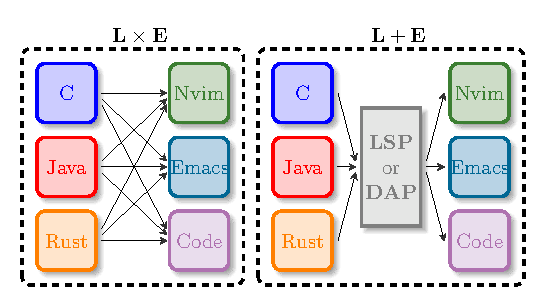
\includegraphics[width=0.75\linewidth]{figs/lsp_combinations.pdf}
    \caption{Traditional approach to language support in editors.}
    \label{fig:traditional}
\end{figure}
In this context, Microsoft in 2016 proposed the \textit{Language Server Protocol} and the \textit{Debugger Adapter Protocol} for Visual Studio Code as a promising solution to this problem, reducing from $\mathcal{L} \times \mathcal{E}$ to $\mathcal{L} + \mathcal{E}$ the number of combinations to be implemented, as it decouples the implementation of the language support from the editor (see Figure~\ref{fig:traditional}).
Detailing, the LSP and DAP are protocols that describes a common \textit{Application Programming Interface} (API) that the \textbf{language server} (LS) should implement, with the benefit of having only one implementation of the LS and multiple clients (IDEs and SCEs) that can consume it, essentially establishing a \textit{client-server} relationship through a communication channel (e.g., \textit{pipes} or \textit{sockets}).
owever, the implementation of an LS and its integration with an IDE/SCEs is still a complex task, as it requires the knowledge of the LSP specification and the implementation of the language support.
The implementation~\cite{Gunasinghe22} of an LS is done entirely manually and it is a \textit{top-down} activity, where most of the time is spent on the design and implementation data structures and algorithms.
Recently, researchers have started talking about the \textit{Software Product Lines} (SPLs) \cite{Cazzola23d, Cazzola20} to move towards a more modular world, where the implementation of a software system can be done in a compositional way, by composing the features of the SPL.
When a SPL is applied to the implementation of a programming language, each product corresponds to a language variant \cite{Cazzola15f} taking the name of \textit{Language Product Lines} (LPLs) \cite{Cazzola15f}. LPLs have been successfully used in both GPLs \cite{Cazzola16, Cazzola16i, Cazzola15f} and DSLs \cite{Haugen08, Liebig13, Cazzola14e, Wende09, White09}.
\hfill \break
\begin{figure}[t]
    \centering
    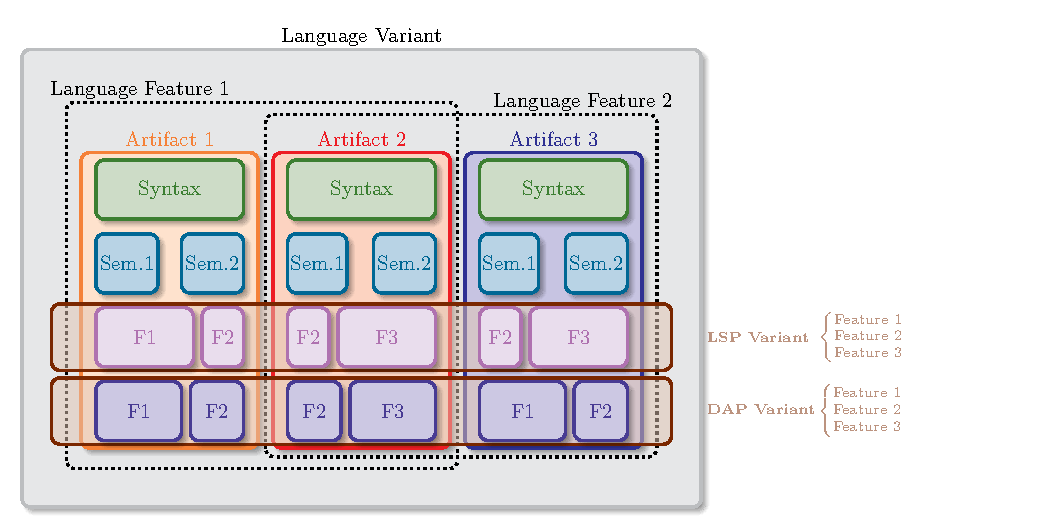
\includegraphics[width=0.9\linewidth]{figs/module_with_lsp.pdf}
    \caption{Proposed approach to modular implementation of LSP and DAP.}
    \label{fig:proposed}
\end{figure}
What I want to prove with this project is that the implementation of an LS could be a \textit{bottom-up} activity, where each LSP or DAP functionality can be see as a separate \textit{feature module} \cite{Batory04, Kastner11} splitted across the language artifacts, where each artifacts can be part of one or more \textit{features} (see Figure~\ref{fig:proposed}). These units can be composed to provide a modular implementation of the LS. This approach is supported by the fact that the LSP and DAP are \textit{language-agnostic} protocol \cite{Niephaus20, Rodriguez-Echeverria18}, which means that it does not impose any restrictions on the implementation of the LS, as long as it respects the specification of the protocol.
In \textit{feature-oriented programming} (FOP) \cite{Apel13, Czarnecki04, Prehofer01}, a feature module is a unit of composition that encapsulates a specific functionality, and it is a first-class entity that can be composed with other feature modules to form a software system; similar to an aspect module that encapsulates a crosscutting concern in \textit{aspect-oriented programming} (AOP) \cite{Kiczales01, Kiczales97, Laddad03}.
So, proponing a new modular approach to the implementation of an LS, based also on FOP, I want to extend Neverlang Language Workbench~\cite{Cazzola15c, Cazzola14c} in order to give support to the implementation of the LS for each semantic action of the language, and I will also implement the Neverlang LSP~\cite{Cazzola19} and DAP to support the composition of the LS feature modules.
In this way, the implementation of the LS is a \textit{bottom-up} activity, where each semantic action has attached a feature module that implements the LS functionality for that action, and these units can be composed to provide a modular implementation of the LS.
Each feature module is written using a DSL, developed in the context of the Neverlang framework, that is specific for the implementation of the LS, and it is independent from the language for which the LS is being implemented.
Furthermore, with this approach, we want to prove that it is possible to reduce the number of combinations from $\mathcal{L} + \mathcal{E}$ to $\mathcal{L} \times 1$ by generating client implementations.

\hfill \break
\noindent
\textbf{Methodology}

The first step involves defining feature modules, which are essential components that encapsulate different functionalities of Language Server Protocol (LSP) and Debug Adapter Protocol (DAP). These functionalities include syntax highlighting, code completion, debugging, and documentation support. Each feature module is identified and defined based on its specific role within the LSP and DAP ecosystem.

Following the identification of feature modules, the next phase is developing domain-specific languages (DSLs) within Neverlang. These DSLs are tailored to facilitate the development and composition of the feature modules, providing a structured and efficient way to create and manage them.

Once the feature modules are defined and the DSLs are developed, the next step is to implement a system within Neverlang that allows for the composition of these feature modules. This system enables the integration of various feature modules into a complete and functional Language Server.

With the modular framework in place, the next phase involves developing Language Servers for multiple programming languages. This step demonstrates the reuse and compositional capabilities of the feature modules. By leveraging the modular design, Language Servers for different languages can be developed more efficiently and with greater consistency.

To ensure the effectiveness of these Language Servers, their performance and integration within different Integrated Development Environments (IDEs) and Source Code Editors (SCEs) will be evaluated. This evaluation will focus on how well the Language Servers perform in real-world development environments and how seamlessly they integrate with existing tools.
Comparison and Analysis

The final phase of the methodology involves a comprehensive comparison and analysis. This includes evaluating the effort and complexity involved in the modular approach compared to traditional top-down methods. By analyzing the development process, the benefits and challenges of using a modular framework can be assessed.

Additionally, the maintainability and extensibility of the modular approach will be scrutinized. This involves introducing changes and enhancements to the Language Servers and observing how easily these modifications can be implemented. The goal is to determine whether the modular approach offers superior maintainability and extensibility compared to traditional methods.

\hfill \break
\noindent
\textbf{Expected Contributions}

\begin{itemize}
    \item \textbf{A Modular Framework for Language Server Development}: A comprehensive framework within the Neverlang Language Workbench that supports the modular development of Language Servers.
    \item \textbf{Reduction in Development Effort}: Empirical evidence demonstrating a reduction in the development effort and complexity associated with implementng Language Servers.
    % \item \textbf{Multiple DSLs for LSP and DAP Development}: Implementation of multiple domain-specific languages (DSLs) specifically designed for developing LSP and DAP functionalities, facilitating easier and more structured creation of Language Servers.
    \item \textbf{Reusable and Language-Agnostic Modules}: A library of reusable, language-agnostic feature modules for common LSP and DAP functionalities.
    \item \textbf{Case Studies and Practical Applications}: Detailed case studies showcasing the practical applications of the modular approach across different programming languages and development environments.
\end{itemize}


\hfill \break
\noindent
\textbf{Timeline of 36 months}

\begin{itemize}
    \item \textbf{Months 1-6}: Literature review on Language Servers, Language Server Protocol, Debug Adapter Protocol, Feature-Oriented Programming, and Software Product Lines.
    \item \textbf{Months 7-12}: Design and development of feature modules for LSP and DAP functionalities within the Neverlang framework.
    \item \textbf{Months 13-18}: Implementation of DSLs for LSP and DAP development, enabling the creation of feature modules.
    \item \textbf{Months 19-24}: Development of a modular system for composing feature modules and generating Language Servers.
    \item \textbf{Months 25-30}: Implementation of Language Servers for multiple programming languages using the modular framework.
    \item \textbf{Months 31-36}: Evaluation of the modular approach, comparison with traditional methods, and analysis of the benefits and challenges.
\end{itemize}

\hfill \break
\noindent
\textbf{Conclusion}

The proposed modular approach to implementing Language Servers via feature-oriented programming within the Neverlang Language Workbench represents a significant advancement in reducing the complexity and effort associated with developing Language Servers. By decomposing the LS functionalities into reusable and composable feature modules, this approach promises to enhance maintainability, extensibility, and overall efficiency in the development of language support tools. This research will contribute valuable insights and practical solutions to the field of programming language implementation and development environment integration.

% \begin{itemize}
%     \item \textbf{Literature Review:} I will perform a literature review on the LSP and DAP, the implementation of the LS, the FOP, and the SPLs.
%     \item \textbf{Design:} I will design the feature modules for the LS, the LSP, and the DAP, and I will extend the Neverlang framework to support the implementation of the LS feature modules.
%     \item \textbf{Implementation:} I will implement the feature modules for the LS, the LSP, and the DAP, and I will extend the Neverlang framework to support the composition of the LS feature modules.
%     \item \textbf{Evaluation:} I will evaluate the proposed approach by implementing the LS for a simple language and by generating the client implementations.
%     \item \textbf{Validation:} I will validate the proposed approach by comparing the implementation of the LS with the traditional approach and by evaluating the generated client implementations.
% \end{itemize}



